\documentclass[assignment3.tex]{subfiles}
\begin{document}

\section*{4η Άσκηση}
Ζητούμενο είναι να προεγγιστούν οι συναρτήσεις $f_1(x)=x^2-2x+3$, $f_2(x)=\cos(\pi x)$ και $f_3(x)=e^{-x}$ με πολυώνυμo δευτέρου βαθμού, οι συντελεστές των όρων του οποίου υπολογίζονται με χρήση της μεθόδου ελαχίστων τετραγώνων.

Έστω ότι το πολυώνυμο που προκύπτει από την μέθοδο ελαχίστων τετραγώνων δίνεται από την εξίσωση \ref{eq:ls_polynomial}, όπου $\lbrace\phi_n(x)\rbrace$ οικογένεια πολυωνύμων που θα χρησιμοποιηθούν σαν βάση για την προσέγγιση. Εν προκειμένω, ζητείται ο βαθμός του πολυωνύμου να είναι $n=2$.

\begin{equation}
p_n(x) = a_0 + a_1 \phi_1(x) + \dots + a_n \phi_n(x)
\label{eq:ls_polynomial}
\end{equation}

Υπάρχουν διάφορες επιλογές για την οικογένεια των πολυωνύμων δευτέρου βαθμού. Η πιο απλή επιλογή είναι τα μονώνυμα $\lbrace1, x, x^2\rbrace$ αλλά υπάρχουν και ορθογώνια πολυώνυμα όπως τα πολυώνυμα \textlatin{Legendre} $\lbrace1, x, x^2-\dfrac{1}{3}\rbrace$. Η μέθοδος ελαχίστων τετραγώνων ελαχιστοποιεί το σφάλμα (\ref{eq:integral_error}).

\begin{equation}
E=\int_{a}^{b} \left[f(x)-P_2(x)\right]^2dx
\label{eq:integral_error}
\end{equation}

Η προσέγγιση με μονώνυμα για το διάστημα $[a,b]$ απαιτεί επίλυση του συστήματος (\ref{eq:ls_monomial_system}), όπου $s_i=\int_{a}^{b}x^idx$ και $b_i=\int_{a}^{b}x^i f(x)dx$. 

\begin{equation}
\left[
\begin{matrix}
s_0 & s_1 & s_2 \\
s_1 & s_2 & s_3 \\
s_2 & s_3 & s_4 \\
\end{matrix}
\right]
\left[
\begin{matrix}
a_0 \\
a_1 \\
a_2 \\
\end{matrix}
\right]=
\left[
\begin{matrix}
b_0 \\
b_1 \\
b_2 \\
\end{matrix}
\right]
\label{eq:ls_monomial_system}
\end{equation}
Για $[a,b]=[0,1]$ o πίνακας είναι ο (\ref{eq:ls_monomial_hilbert}), ο πίνακας \textlatin{Hilbert}, ο οποίος είναι αντιστρέψιμος για $n=3$, για μεγαλύτερα $n$ οδηγεί σε ασταθή συστήματα.
\begin{equation}
S=\left[
\begin{matrix}
1 & \frac{1}{2} & \frac{1}{3} \\
\frac{1}{2} & \frac{1}{3} & \frac{1}{4} \\
\frac{1}{3} & \frac{1}{4} & \frac{1}{5} \\
\end{matrix}
\right]
\label{eq:ls_monomial_hilbert}
\end{equation}
Για το λόγο αυτό, σε μεγαλύτερα $n$ χρησιμοποιούνται ορθογώνια πολυώνυμα, όπως τα \textlatin{Legendre}. Τα ορθογώνια πολυώνυμα μηδενίζουν όλα τα μη διαγώνια στοιχεία του Πίνακα \ref{eq:ls_monomial_system} και η επίλυσή του είναι άμεση.
Συγκεκριμένα, είναι $s_i = \int_{a}^{b}w(x)\phi_i^2(x)dx$ και $b_i=\int_{a}^{b}w(x)\phi_i(x) f(x)dx$, όπου $w(x)=1$ κατάληλλη συνάρτηση βάρους. 

Σε αντίθεση με την περίπτωση των μονώνυμων, η ολοκλήρωση πρέπει να γίνει στο διάστημα $[-1,1]$, για να ισχύει η σχέση ορθογωνιότητας (\ref{eq:orthogonality}). Το ζητούμενο διάστημα προσέγγισης εξακολουθεί να είναι το $[0,1]$ καθώς είναι υποσύνολο του $[-1,1]$.
\begin{equation}
\int_{-1}^{1}\phi_i(x)\phi_j(x)dx=0
\label{eq:orthogonality}
\end{equation}

Για σύγκριση, το πρόβλημα λύνεται υπολογιστικά και με τις δύο προσεγγίσεις. Και στις δύο περιπτώσεις, αναμένεται για κάθε συνάρτηση $f_k(x)$ να παραχθεί ένα πολυώνυμο δευτέρου βαθμού. Ειδικότερα, η $f_1(x)$ είναι ήδη ένα πολυώνυμο δευτέρου βαθμού και επομένως αναμένεται η μέθοδος ελαχίστων τετραγώνων να παράγει σαν πολυώνυμο την ίδια την $f_1(x)$.

Στα Σχήματα \ref{fig:lsquares_1}, \ref{fig:lsquares_2} και \ref{fig:lsquares_3} φαίνονται τα αποτελέσματα της προσέγγισης. Όπως ήταν αναμενόμενο, η μέθοδος ελαχίστων τετραγώνων παράγει την ίδια την $f_1(x)$ στην πρώτη περίπτωση. Επίσης, στην δεύτερη περίπτωση, η λύση με μονώνυμα είναι μια ευθεία σε αντίθεση με την λύση με πολυώνυμα \textlatin{Legendre}, που είναι δευτέρου βαθμού.

\begin{figure}[hp]
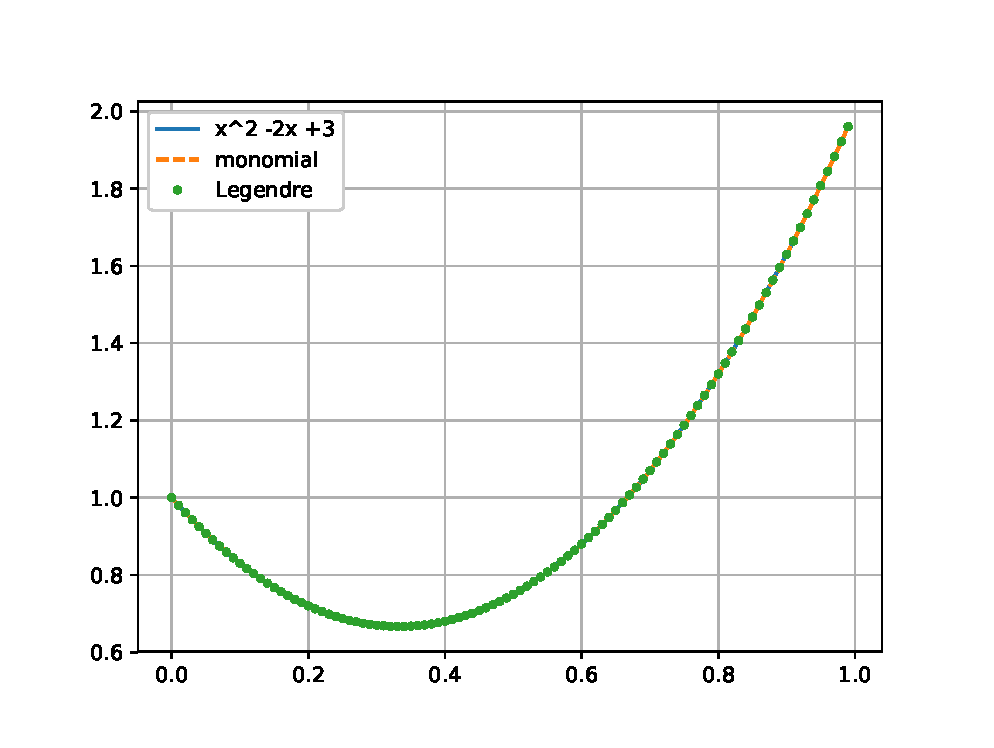
\includegraphics[width=0.7\textwidth]{lsquares_1.eps}
\centering
\caption{Ελάχιστα Τετράγωνα για $x^2-2x+3$}
\label{fig:lsquares_1}
\end{figure}

\begin{figure}[hp]
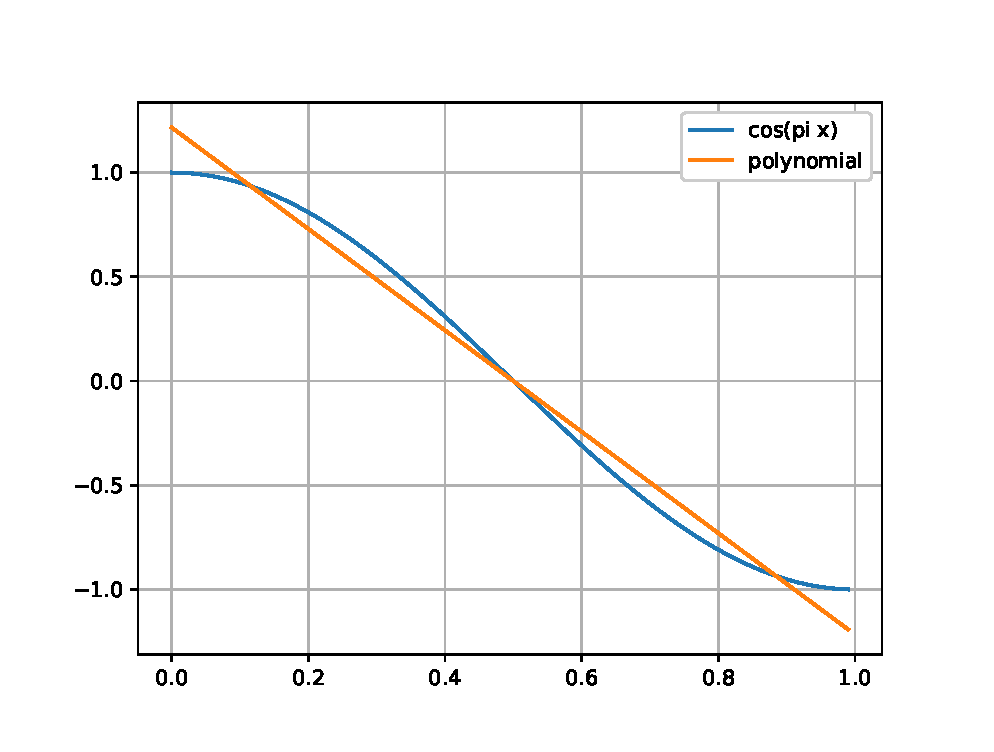
\includegraphics[width=0.7\textwidth]{lsquares_2.eps}
\centering
\caption{Ελάχιστα Τετράγωνα για $\cos(\pi x)$}
\label{fig:lsquares_2}
\end{figure}

\begin{figure}[hp]
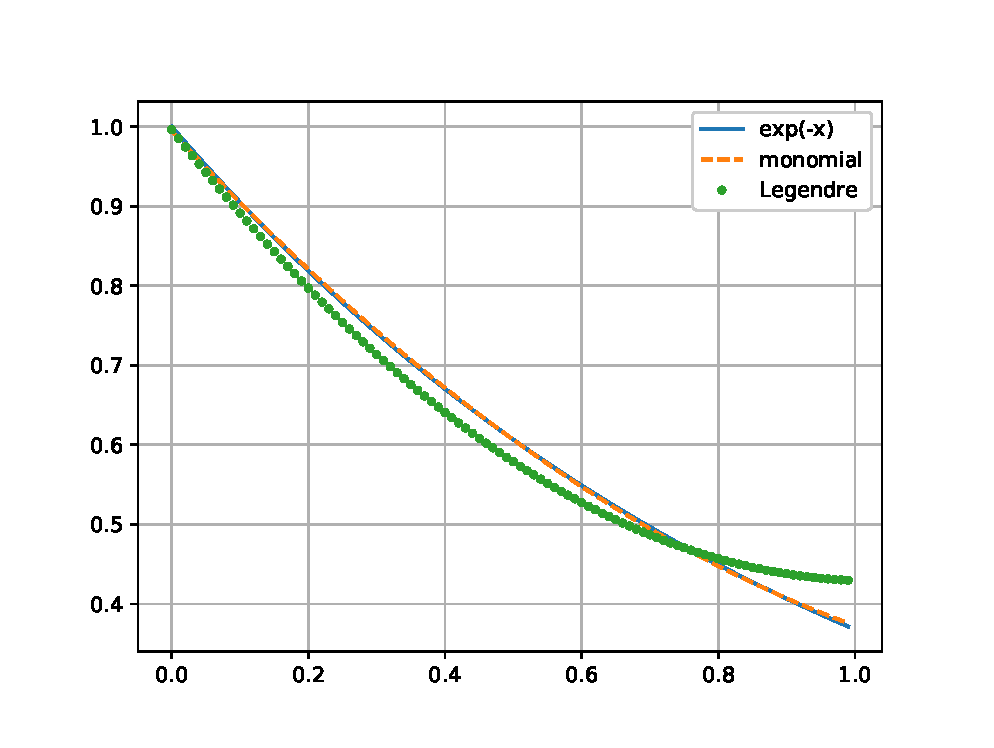
\includegraphics[width=0.7\textwidth]{lsquares_3.eps}
\centering
\caption{Ελάχιστα Τετράγωνα για $e^{-x}$}
\label{fig:lsquares_3}
\end{figure}

Παρακάτω ακολουθεί ο κώδικας που γράφτηκε σε \textlatin{Python} και έγινε χρήση της βιβλιοθήκης \textlatin{Numpy}. Οι ρουτίνες ελαχίστων τετραγώνων με μονώνυμα και με πολυώνυμα \textlatin{Legendre} δίνονται στο Παράρτημα.
\selectlanguage{english}
\lstinputlisting[style=python, firstline=8]{ex4.py}
\end{document}